%%%%%%%%%%%%%%%%%%%%%%%%%%%%%%%%%%%%%%%%%%%%%%%%%%%%%%%%%%%%%%%%%%%%%%%%%%%%%%%%
%                                                                              %
%                    PLANTILLA DE PRESENTACIÓN BEAMER                          %
%                                                                              %
%  Esta plantilla usa la clase beamer para crear presentaciones académicas.    %
%  Incluye un entorno personalizado 'caja' para resaltar contenido.            %
%                                                                              %
%%%%%%%%%%%%%%%%%%%%%%%%%%%%%%%%%%%%%%%%%%%%%%%%%%%%%%%%%%%%%%%%%%%%%%%%%%%%%%%%

\documentclass{beamer}

%===============================================================================
%                      CONFIGURACIÓN DEL TEMA
%===============================================================================
\mode<presentation>

% --- Tema visual ---
% Opciones populares: Madrid, AnnArbor, Berlin, Copenhagen, Darmstadt
\usetheme{AnnArbor}

% --- Esquema de colores ---
% Opciones: beaver, crane, dolphin, lily, orchid, rose, seagull, whale
\usecolortheme{dolphin}

% --- Imagen de fondo (opcional) ---
% Comenta esta línea si no quieres imagen de fondo
\setbeamertemplate{background canvas}{%
    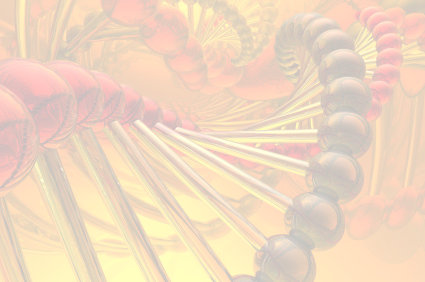
\includegraphics[width=\paperwidth,height=\paperheight]{fotos/fondo.jpg}%
}

%===============================================================================
%                         PAQUETES
%===============================================================================
\usepackage[spanish]{babel}     % Idioma español
\usepackage[utf8]{inputenc}     % Codificación UTF-8
\usepackage{multicol}           % Múltiples columnas
\usepackage{xypic}              % Diagramas (si necesario)

%===============================================================================
%                    ENTORNO PERSONALIZADO: CAJA
%===============================================================================
% Define colores para las cajas
\setbeamercolor{upcol}{fg=blue,bg=orange}       % Cabecera: texto azul, fondo naranja
\setbeamercolor{lowcol}{fg=black,bg=blue!20}    % Cuerpo: texto negro, fondo azul claro

% Entorno 'caja' basado en beamerboxesrounded
% Uso: \begin{caja}{Título de la caja} contenido... \end{caja}
\newenvironment{caja}[1]{%
    \begin{beamerboxesrounded}[upper=upcol,lower=lowcol,shadow=true]{#1}%
}{%
    \end{beamerboxesrounded}%
}

%===============================================================================
%                      DATOS DE LA PRESENTACIÓN
%===============================================================================
\title{Título de la Presentación}
\author{Nombre Autor \\ \texttt{email@ugr.es}}
\institute[]{%
    Departamento\\
    Universidad de Granada
}
\date{Curso 20XX-20XX}

%===============================================================================
%                         DOCUMENTO
%===============================================================================
\begin{document}

%-------------------------------------------------------------------------------
% Diapositiva de título
%-------------------------------------------------------------------------------
\begin{frame}
    \titlepage
\end{frame}

%-------------------------------------------------------------------------------
% Índice de contenidos
%-------------------------------------------------------------------------------
\begin{frame}
    \frametitle{Contenidos}
    \tableofcontents
\end{frame}

%===============================================================================
%                          SECCIÓN 1
%===============================================================================
\section{Primera Sección}

%-------------------------------------------------------------------------------
\begin{frame}
    \frametitle{Título de la Diapositiva}
    \framesubtitle{Subtítulo opcional}
    
    \begin{caja}{Concepto Principal}
        \begin{itemize}
            \item<1-> Primer punto (aparece desde overlay 1)
            \item<2-> Segundo punto (aparece desde overlay 2)
            \item<3-> Tercer punto (aparece desde overlay 3)
            \item<4> Cuarto punto (solo visible en overlay 4)
        \end{itemize}
    \end{caja}
\end{frame}

%-------------------------------------------------------------------------------
\begin{frame}
    \frametitle{Ejemplo con Alertas}
    \framesubtitle{Resaltado secuencial}
    
    \begin{caja}{Items con alerta}
        % [<+-| alert@+>] hace que cada item aparezca y se resalte secuencialmente
        \begin{itemize}[<+-| alert@+>]
            \item Este item se resalta cuando aparece
            \item Luego este se resalta
            \item Y finalmente este
        \end{itemize}
    \end{caja}
\end{frame}

%-------------------------------------------------------------------------------
\begin{frame}
    \frametitle{Imagen Centrada}
    
    \begin{center}
        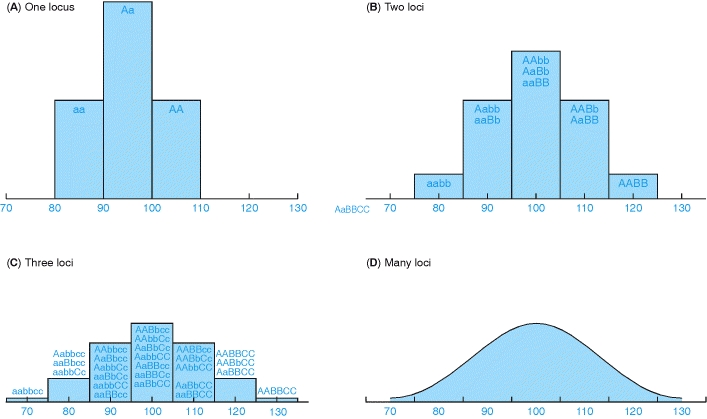
\includegraphics[width=0.8\textwidth]{fotos/ch19f1}
    \end{center}
\end{frame}

%===============================================================================
%                          SECCIÓN 2
%===============================================================================
\section{Segunda Sección}

%-------------------------------------------------------------------------------
\begin{frame}
    \frametitle{Diseño en Columnas}
    \framesubtitle{Texto e imagen lado a lado}
    
    \begin{columns}
        \begin{column}{0.4\textwidth}
            \begin{caja}{Concepto}
                El texto explicativo va aquí.
                Puede incluir fórmulas: $E = mc^2$
            \end{caja}
        \end{column}
        \hfill
        \begin{column}{0.55\textwidth}
            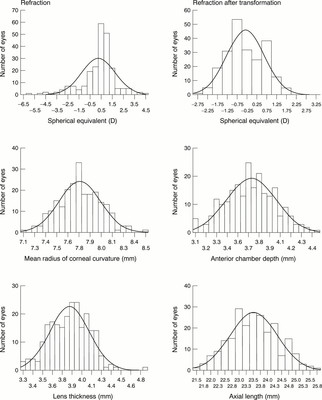
\includegraphics[width=0.9\textwidth]{fotos/distribucion.jpg}
        \end{column}
    \end{columns}
\end{frame}

%-------------------------------------------------------------------------------
\begin{frame}
    \frametitle{Uso de pause}
    \framesubtitle{Revelado progresivo simple}
    
    \begin{caja}{Conceptos}
        Primer concepto importante.
        \pause
        
        Segundo concepto que aparece después.
        \pause
        
        Tercer concepto final.
    \end{caja}
\end{frame}

%===============================================================================
%                          SECCIÓN 3
%===============================================================================
\section{Resumen}

%-------------------------------------------------------------------------------
\begin{frame}
    \frametitle{Conclusiones}
    
    \begin{caja}{Resumen}
        \begin{enumerate}
            \item Primera conclusión
            \item Segunda conclusión
            \item Tercera conclusión
        \end{enumerate}
    \end{caja}
    
    \vspace{1em}
    
    \begin{center}
        \Large ¡Gracias por su atención!
    \end{center}
\end{frame}

\end{document}

%===============================================================================
%                    PLANTILLAS DE DIAPOSITIVAS
%===============================================================================
% Las siguientes plantillas están después de \end{document}, por lo que LaTeX
% las ignora. Puedes copiarlas y pegarlas directamente en tu presentación.

% --- Diapositiva simple ---
\begin{frame}
    \frametitle{Título}
    \framesubtitle{Subtítulo}
    
    Contenido aquí...
\end{frame}

% --- Diapositiva con columnas ---
\begin{frame}
    \frametitle{Título}
    \begin{columns}
        \begin{column}{0.5\textwidth}
            Columna izquierda
        \end{column}
        \begin{column}{0.5\textwidth}
            Columna derecha
        \end{column}
    \end{columns}
\end{frame}

% --- Diapositiva con caja personalizada ---
\begin{frame}
    \frametitle{Título}
    \begin{caja}{Título de la caja}
        Contenido de la caja...
    \end{caja}
\end{frame}

% --- Diapositiva con imagen y texto ---
\begin{frame}
    \frametitle{Título}
    \begin{columns}
        \begin{column}{0.4\textwidth}
            Texto explicativo aquí.
        \end{column}
        \begin{column}{0.55\textwidth}
            \includegraphics[width=\textwidth]{imagen}
        \end{column}
    \end{columns}
\end{frame}

% --- Diapositiva con lista animada ---
\begin{frame}
    \frametitle{Título}
    \begin{itemize}[<+-| alert@+>]
        \item Primer punto
        \item Segundo punto
        \item Tercer punto
    \end{itemize}
\end{frame}
